% !TEX TS-program = lualatex
% !BIB TS-program = biber
%\documentclass[handout]{beamer}
\documentclass{beamer}
\input{../common/misomva}\usetikzlibrary{decorations.pathmorphing}
%\newcommand{\misoclasstinytitleslide}{Partially based on material by:  Ulrike von Luxburg, \\[-1em] Gary Miller, Doyle \& Schnell, Daniel Spielman}
\newcommand{\misoclasstinytitleslide}{Partially based on material by:   Gary Miller, \\ Mikhail Belkin, Branislav Kveton, \\[-1em] Doyle \& Schnell, Daniel Spielman}
\newcommand{\misoclassdate}{}
\begin{document}
% Topic-specific title slide
\newcommand{\topictitle}{SSL with Graphs: Harmonic Functions}
\newcommand{\topicsubtitle}{Gaussian Random Fields Solution}
\renewcommand{\misoclasstinytitleslide}{Partially based on material by:  Mikhail Belkin, Partha Niyogi, \\[-1em] Olivier Chapelle, Bernhard Sch\"olkopf}

\MakeTopicSlide

\begin{frame}
\frametitle{SSL with Graphs: Harmonic Functions}

{\small Zhu/Ghahramani/Lafferty: Semi-Supervised Learning Using Gaussian Fields and Harmonic Functions \textsc{(ICML 2013)}}
{\scriptsize 
\url{http://mlg.eng.cam.ac.uk/zoubin/papers/zgl.pdf}
}
\pause \\
\grcol{\tiny *a seminal paper that convinced people to use graphs for SSL}

\pause

\textbf{Idea 1:} Look for a \emphcol{unique} solution. \\
\pause
\textbf{Idea 2:} Find a smooth one. \pause (\emphcol{harmonic} solution) \\

\pause 

\emphcol{Harmonic SSL}

\textbf{1):} As before, we constrain $f$ to match the supervised data: \pause
$$
f(\bx_i) = y_i \qquad \forall i \in \{1, \dots, n_l \}
$$
\pause
\textbf{2):} We enforce the solution $f$ to be harmonic: \pause
$$
f(\bx_i) = \frac{\sum_{i\sim j} f(\bx_j)w_{ij}}{\sum_{i\sim j}   w_{ij}} \qquad \forall i \in \{n_l+1, \dots, n_u+n_l \}
$$
% 
% 
% 
% $$

\end{frame}
%%%%%%%%%%%%%%%%%%%%%%%%%%%%%%%%%%%%%%%%%%%%%%%%%%%%%%%%%%%%


\begin{frame}
\frametitle{SSL with Graphs: Harmonic Functions}

The harmonic solution is obtained from the mincut one \dots \pause

  $$
   \min_{\bff  \in \{\pm 1\}^{n_l + n_u} }\mcolA{\infty \sum_{i=1}^{n_l} \left( f(\bx_i) - y_i \right)^2}
   + \lambda\mcolB{\sum_{i,j=1}^{n_l+n_u} w_{ij} \left( f(\bx_i)  - f(\bx_j)  \right)^2}
  $$

\pause
\dots if we just relax the integer constraints to be real \dots
\pause
  
  $$
   \min_{\bff  \in \alert{\R^{n_l + n_u}} }\mcolA{\infty \sum_{i=1}^{n_l} \left( f(\bx_i) - y_i \right)^2}
   + \lambda\mcolB{\sum_{i,j=1}^{n_l+n_u} w_{ij} \left( f(\bx_i)  - f(\bx_j)  \right)^2}
  $$
\pause
\dots or equivalently  (note that $f(\bx_i) = f_i$) \dots
\pause
\begin{align*}
\min_{\bff \in \R^{n_l + n_u} }
   &  \mcolB{\sum_{i,j=1}^{n_l+n_u} w_{ij} \left( f(\bx_i)  - f(\bx_j)  \right)^2} \\
 s.t. \quad & \mcolA{y_i  = f(\bx_i)}   \quad \forall i = 1,\dots,n_l
\end{align*}


\end{frame}
%%%%%%%%%%%%%%%%%%%%%%%%%%%%%%%%%%%%%%%%%%%%%%%%%%%%%%%%%%%%
\begin{frame}
\frametitle{SSL with Graphs: Harmonic Functions}

\textbf{Properties of the relaxation from $\pm 1$ to $\R$ }

\begin{itemize}%\addtolength{\itemsep}{0.75\baselineskip}
\item there is a closed form solution for $\bff$
\item this solution is unique
\item globally optimal
%\item it is either constant or has a maximum/minimum on a boundary
\pause
\item $f(\bx_i)$ may not be discrete 
\begin{itemize}
\item but we can threshold it 
\end{itemize}
\pause
\item electric-network interpretation
\item random-walk interpretation
\end{itemize}

\end{frame}
%%%%%%%%%%%%%%%%%%%%%%%%%%%%%%%%%%%%%%%%%%%%%%%%%%%%%%%%%%%%
\begin{frame}
\frametitle{SSL with Graphs: Harmonic Functions}
\vskip -1em
\begin{center}
\resizebox{\columnwidth}{!}{%
\begin{tikzpicture}[
    unlabeled/.style={circle, draw=black, thick, minimum size=10pt, fill=white},
    labeled1/.style={circle, draw=orange, very thick, minimum size=12pt, fill=black},
    labeled0/.style={circle, draw=orange, very thick, minimum size=12pt, fill=white},
    labeledi/.style={circle, draw=orange, very thick, minimum size=12pt, fill=yellow},
    edge/.style={draw=black, thin}
]

    % ===== LEFT PANEL: Electric Network Interpretation =====
    \begin{scope}[xshift=0cm]
        
        % Resistor symbol
        \draw[thick] (-3.5, 3.5) -- (-3.2, 3.5);
        \draw[thick, decorate, decoration={zigzag, segment length=2mm, amplitude=1mm}] (-3.2, 3.5) -- (-2.2, 3.5);
        \draw[thick] (-2.2, 3.5) -- (-1.9, 3.5);
        
        % R_ij = 1/w_ij formula
        \node[font=\itshape] at (-2.7, 2.8) {$R_{ij} = \dfrac{1}{w_{ij}}$};
        
        % Graph nodes - S shape
        % Upper arc
        \node[unlabeled] (a1) at (0.5, 4) {};
        \node[unlabeled] (a2) at (1.2, 4.3) {};
        \node[labeled1] (n1) at (1.9, 4.1) {};  % Node 1
        \node[unlabeled] (a3) at (2.6, 4.3) {};
        \node[unlabeled] (a4) at (3.3, 4.0) {};
        \node[unlabeled] (a5) at (3.8, 3.5) {};
        \node[unlabeled] (a6) at (4.0, 2.9) {};
        
        % Upper arc inner
        \node[unlabeled] (b1) at (0.8, 3.3) {};
        \node[unlabeled] (b2) at (1.5, 3.5) {};
        \node[unlabeled] (b3) at (2.2, 3.4) {};
        \node[unlabeled] (b4) at (2.9, 3.5) {};
        \node[unlabeled] (b5) at (3.4, 3.1) {};
        \node[unlabeled] (b6) at (3.6, 2.5) {};
        
        % Middle connector and node 0
        \node[unlabeled] (c1) at (2.0, 2.7) {};
        \node[unlabeled] (c2) at (2.7, 2.5) {};
        \node[labeled0] (n0) at (3.4, 2.0) {};  % Node 0
        
        % Lower arc
        \node[unlabeled] (d1) at (1.5, 2.2) {};
        \node[unlabeled] (d2) at (2.2, 1.8) {};
        \node[unlabeled] (d3) at (2.9, 1.5) {};
        \node[unlabeled] (d4) at (2.5, 0.9) {};
        \node[unlabeled] (d5) at (1.8, 0.6) {};
        \node[unlabeled] (d6) at (1.1, 0.5) {};
        \node[unlabeled] (d7) at (0.4, 0.7) {};
        
        % Lower arc outer
        \node[unlabeled] (e1) at (1.2, 1.5) {};
        \node[unlabeled] (e2) at (1.9, 1.1) {};
        \node[unlabeled] (e3) at (2.2, 0.5) {};
        \node[unlabeled] (e4) at (1.5, 0.1) {};
        \node[unlabeled] (e5) at (0.8, 0.0) {};
        \node[unlabeled] (e6) at (0.1, 0.2) {};
        
        % Minimal edges to show structure without clutter
        \draw[edge, opacity=0.3] (a1) -- (a2) -- (n1) -- (a3) -- (a4) -- (a5) -- (a6);
        \draw[edge, opacity=0.3] (b1) -- (b2) -- (b3) -- (b4) -- (b5) -- (b6);
        \draw[edge, opacity=0.3] (c1) -- (c2) -- (n0);
        \draw[edge, opacity=0.3] (d1) -- (d2) -- (d3) -- (n0);
        \draw[edge, opacity=0.3] (d3) -- (d4) -- (d5) -- (d6) -- (d7);
        
        % Battery/voltage source - directly connected to orange-outlined nodes
        % Wire from node 1 (orange outline) going right to battery
        \draw[thick] (n1) -- (4.5, 4.1);
        \draw[thick] (4.5, 4.1) -- (4.5, 3.4);
        % Battery plates
        \draw[very thick] (4.3, 3.4) -- (4.7, 3.4);  % Long plate (+)
        \draw[thick] (4.35, 3.2) -- (4.65, 3.2);  % Short plate (-)
        % Wire from battery to node 0 (orange outline)
        \draw[thick] (4.5, 3.2) -- (4.5, 2.0) -- (n0);
        % +1 volt label
        \node[font=\large] at (5.3, 3.3) {+1 volt};
        
        % Labels
        \node[font=\bfseries] at (1.9, 3.5) {1};
        \node[font=\bfseries] at (3.9, 2.0) {0};
        
        % Caption
        \node[font=\large] at (1.5, -0.7) {(a) The electric network interpretation};
    \end{scope}
    
    % ===== RIGHT PANEL: Random Walk Interpretation =====
    \begin{scope}[xshift=8cm]
        
        % Graph nodes - S shape (same structure)
        % Upper arc
        \node[unlabeled] (ra1) at (0.5, 4) {};
        \node[unlabeled] (ra2) at (1.2, 4.3) {};
        \node[labeled1] (rn1) at (1.9, 4.1) {};  % Node 1
        \node[unlabeled] (ra3) at (2.6, 4.3) {};
        \node[unlabeled] (ra4) at (3.3, 4.0) {};
        \node[unlabeled] (ra5) at (3.8, 3.5) {};
        \node[unlabeled] (ra6) at (4.0, 2.9) {};
        
        % Upper arc inner
        \node[unlabeled] (rb1) at (0.8, 3.3) {};
        \node[unlabeled] (rb2) at (1.5, 3.5) {};
        \node[unlabeled] (rb3) at (2.2, 3.4) {};
        \node[unlabeled] (rb4) at (2.9, 3.5) {};
        \node[unlabeled] (rb5) at (3.4, 3.1) {};
        \node[unlabeled] (rb6) at (3.6, 2.5) {};
        
        % Middle connector and node 0
        \node[unlabeled] (rc1) at (2.0, 2.7) {};
        \node[unlabeled] (rc2) at (2.7, 2.5) {};
        \node[labeled0] (rn0) at (3.4, 2.0) {};  % Node 0
        
        % Lower arc
        \node[unlabeled] (rd1) at (1.5, 2.2) {};
        \node[unlabeled] (rd2) at (2.2, 1.8) {};
        \node[unlabeled] (rd3) at (2.9, 1.5) {};
        \node[unlabeled] (rd4) at (2.5, 0.9) {};
        \node[labeledi] (rni) at (1.8, 0.6) {};  % Node i (yellow)
        \node[unlabeled] (rd6) at (1.1, 0.5) {};
        \node[unlabeled] (rd7) at (0.4, 0.7) {};
        
        % Lower arc outer
        \node[unlabeled] (re1) at (1.2, 1.5) {};
        \node[unlabeled] (re2) at (1.9, 1.1) {};
        \node[unlabeled] (re3) at (2.2, 0.5) {};
        \node[unlabeled] (re4) at (1.5, 0.1) {};
        \node[unlabeled] (re5) at (0.8, 0.0) {};
        \node[unlabeled] (re6) at (0.1, 0.2) {};
        
        % Regular edges
        \draw[edge] (ra1) -- (ra2) -- (rn1) -- (ra3) -- (ra4) -- (ra5) -- (ra6);
        \draw[edge] (rb1) -- (rb2) -- (rb3) -- (rb4) -- (rb5) -- (rb6);
        \draw[edge] (ra1) -- (rb1); \draw[edge] (ra2) -- (rb2);
        \draw[edge] (rn1) -- (rb3); \draw[edge] (ra3) -- (rb4);
        \draw[edge] (ra4) -- (rb5); \draw[edge] (ra5) -- (rb6);
        \draw[edge] (rb3) -- (rc1) -- (rc2) -- (rn0);
        \draw[edge] (rb5) -- (rc2);
        \draw[edge] (rb6) -- (rn0);
        \draw[edge] (rc1) -- (rd1) -- (rd2) -- (rd3) -- (rn0);
        \draw[edge] (rd3) -- (rd4) -- (rni) -- (rd6) -- (rd7);
        \draw[edge] (re1) -- (re2) -- (re3) -- (re4) -- (re5) -- (re6);
        \draw[edge] (rd1) -- (re1); \draw[edge] (rd2) -- (re2);
        \draw[edge] (rd4) -- (re3); \draw[edge] (rni) -- (re4);
        \draw[edge] (rd6) -- (re5); \draw[edge] (rd7) -- (re6);
        
        % Green path (from i toward 1 - going around UPPER arc)
        % From i up through lower arc
        \draw[green!70!black, line width=2pt, ->] (rni) -- (rd4);
        \draw[green!70!black, line width=2pt, ->] (rd4) -- (rd3);
        \draw[green!70!black, line width=2pt, ->] (rd3) -- (rd2);
        \draw[green!70!black, line width=2pt, ->] (rd2) -- (rd1);
        \draw[green!70!black, line width=2pt, ->] (rd1) -- (rc1);
        % Up to inner upper arc
        \draw[green!70!black, line width=2pt, ->] (rc1) -- (rb3);
        \draw[green!70!black, line width=2pt, ->] (rb3) -- (rb2);
        \draw[green!70!black, line width=2pt, ->] (rb2) -- (rb1);
        % Around outer upper arc to node 1
        \draw[green!70!black, line width=2pt, ->] (rb1) -- (ra1);
        \draw[green!70!black, line width=2pt, ->] (ra1) -- (ra2);
        \draw[green!70!black, line width=2pt, ->] (ra2) -- (rn1);
        
        % Blue path (from i going other direction through lower outer arc)
        \draw[blue!70, line width=2pt, ->] (rni) -- (re4);
        \draw[blue!70, line width=2pt, ->] (re4) -- (re5);
        \draw[blue!70, line width=2pt, ->] (re5) -- (re6);
        \draw[blue!70, line width=2pt, ->] (re6) -- (rd7);
        \draw[blue!70, line width=2pt, ->] (rd7) -- (rd6);
        
        % Pink arrows (toward 0)
        \draw[magenta, line width=1.5pt, ->] (rc2) -- (rn0);
        \draw[magenta, line width=1.5pt, ->] (rd3) -- (rn0);
        
        % Labels
        \node[font=\bfseries] at (1.9, 3.5) {1};
        \node[font=\bfseries] at (3.9, 2.0) {0};
        \node[font=\itshape] at (2.3, 0.6) {$i$};
        
        % Caption
        \node[font=\large] at (1.5, -0.7) {(b) The random walk interpretation};
    \end{scope}
    
\end{tikzpicture}
}
{\tiny Figure from \citet{zhu2003semi-supervised}}
\end{center}
\vskip -1em
\pause
\textbf{Random walk interpretation}: \\
\textbf{1)} start from the vertex you want to label and randomly walk\\
\pause
\textbf{2)} $P(j|i) = \frac{w_{ij}}{\sum_k w_{ik}}$ 
\pause \qquad $\equiv$ \qquad $\bP = \bD^{-1}\bW$\\
\pause
\textbf{3)} finish when \textbf{a} labeled vertex is hit 
\pause
\begin{center}
\vskip -1em
\emphcol{absorbing random walk}
\end{center}
\vskip -1em
$f_i = $ \pause probability of reaching \alert{a} positive labeled vertex
\end{frame}
%%%%%%%%%%%%%%%%%%%%%%%%%%%%%%%%%%%%%%%%%%%%%%%%%%%%%%%%%%%%
\begin{frame}
\frametitle{SSL with Graphs: Harmonic Functions}
\questionbox{How to compute HS?}
\pause
\textbf{Option A:} iteration\pause/propagation \\[1em]
\pause
\textbf{Step 1:} Set $f(\bx_i) = y_i$ for $i=1,\dots,n_l$ \\
\pause
\textbf{Step 2:} Propagate iteratively (only for unlabeled)
 $$
f(\bx_i) \gets \frac{\sum_{i\sim j} f(\bx_j)w_{ij}}{\sum_{i\sim j} w_{ij}} \qquad \forall i \in \{n_l+1, \dots, n_u+n_l \}
$$
\pause

Properties:
\begin{itemize}
[<+->]%\addtolength{\itemsep}{0.75\baselineskip}
\item this will converge to the harmonic solution
\item we can set the initial values for unlabeled nodes arbitrarily
\item an interesting option for large-scale data
\end{itemize}


\end{frame}

%%%%%%%%%%%%%%%%%%%%%%%%%%%%%%%%%%%%%%%%%%%%%%%%%%%%%%%%%%%%
\begin{frame}
\frametitle{SSL with Graphs: Harmonic Functions}
\questionbox{How to compute HS?}
\textbf{Option B:} Closed form solution \pause \\[1em]
Define $\bff = (f(\bx_1), \dots, f(\bx_{n_l + n_u})) 
\pause =
(f_1, \dots, f_{n_l + n_u})$
\pause
$$
\Omega(\bff) = 
\pause 
\mcolB{\sum_{i,j=1}^{n_l+n_u} w_{ij} \left( f(\bx_i)  - f(\bx_j)  \right)^2}
\pause 
= \bff\transpose\bL\bff
$$

$\bL$ is a $\left(n_l + n_u\right) \times \left(n_l + n_u\right)$ matrix: \pause

$$
 \bL = 
\left[\begin{array}{cc}
\bL_{ll}  & \bL_{lu}\\
\bL_{ul} & \bL_{uu}\\
\end{array}\right]
$$
\pause 
\questionbox{How to compute this \textbf{constrained} minimization problem?} \\
\pause
\onslide<handout:0>{\notecol{%
\tiny \qquad Yes, Lagrangian multipliers are an option, but $\dots$}}
\end{frame}
%%%%%%%%%%%%%%%%%%%%%%%%%%%%%%%%%%%%%%%%%%%%%%%%%%%%%%%%%%%%
\begin{frame}
\frametitle{SSL with Graphs: Harmonic Functions}
\rightyellbox{Let us compute \textbf{harmonic} solution using \textbf{harmonic} property!}
\pause
%\pause
$$\left(\bL\bff \right)_u = \bZero_{u}$$ \\
\pause
In matrix notation
$$
\left[\begin{array}{cc}
\bL_{ll}  & \bL_{lu}\\
\bL_{ul} & \bL_{uu}\\
\end{array}\right]
\left[\begin{array}{c}
\bff_{l} \\
\bff_{u} \\
\end{array}\right]
=
\left[\begin{array}{cc}
\dots\\
\bZero_{u}\\
\end{array}\right]
$$
\pause
$\bff_{l}$ is constrained to be $\by_l$ and for $\bff_{u}$ \dots
\dots
$$
 \bL_{ul}\bff_{l} + \bL_{uu}\bff_{u} = \bZero_{u}
$$
\pause \dots from which we get 
$$
 \bff_{u} = \bL_{uu}^{-1}(-\bL_{ul}\bff_{l}) \pause = 
 \bL_{uu}^{-1}(\bW_{ul}\bff_{l}).
 \pause
 \quad\quad \text{\notecol{$\bL_{ul} = \mathbf{0} - \bW_{ul}$}}
$$
\pause
\vspace{-2em}
\begin{flushright}
\notecol{\small  Note that $\bff_u$ does not depend on $\bL_{ll}$. }
\end{flushright}
\end{frame}

%%%%%%%%%%%%%%%%%%%%%%%%%%%%%%%%%%%%%%%%%%%%%%%%%%%%%%%
%%%%%%%%%%%%%%%%%%%%%%%%%%%%%%%%%%%%%%%%%%%%%%%%%%%%%%%%%%%%
\begin{frame}
\frametitle{SSL with Graphs: Harmonic Functions}
\rightquestionbox{Can we see that this calculates the probability of a random walk?}
$$
 \bff_{u} = \bL_{uu}^{-1}(-\bL_{ul}\bff_{l}) \pause = 
 \bL_{uu}^{-1}(\bW_{ul}\bff_{l})
$$
\pause
Note $\bP = \bD^{-1}\bW$ and $\bL_{uu}^{-1} = (\bD_{uu}(\bI - \bP_{uu}))^{-1} = (\bI - \bP_{uu})^{-1}\bD_{uu}^{-1}$ \pause
\begin{align*}
  \bff_{u} = (\bI -  \bP_{uu})^{-1} \bP_{ul} \bff_l.
  %\label{eq:random walk HFS}
\end{align*}
\pause
Split the equation into +ve \& -ve part:
\begin{align*}
  f_i
  \ = & \ \ \action<+->{(\bI - \bP_{uu})_{iu}^{-1} \bP_{ul} \bff_l} \nonumber \\
  \ \action<+->{= & \ \
  \underbrace{\sum_{j: y_j = 1} (\bI - \bP_{uu})_{iu}^{-1}
  \bP_{uj}}_{p_i^{(+1)}} -
  \underbrace{\sum_{j: y_j = -1} (\bI - \bP_{uu})_{iu}^{-1}
  \bP_{uj}}_{p_i^{(-1)}} } \nonumber \\
  \ \action<+->{= & \ \ p_i^{(+1)} - p_i^{(-1)}}
  %\label{eq:probability HFS}
\end{align*}

\end{frame}


\MakeLastSlide
\end{document}
